\chapter{Pruebas a la extensi\'on de Pakal y sus Resultados}

Para probar la extensi\'on realizada al modelo computacional Pakal, se llevaron a cabo las simulaci\'ones del comportamiento de los campos magn\'eticos seg\'un dos modelos distintos: uno en forma de arco magn\'etico \citep{ashwanden} y otro en forma de un flujo emergente \citep{flujoemergente}. A continuaci\'on se precisar\'an las caracter\'isticas f\'isicas en cada modelo; as\'i como los resultados obtenidos para cada caso tras.

\section{Caracter\'isticas F\'isicas de los modelos de prueba \- Arcos Magn\'eticos y Flujo Emergente}

Se eligieron dos modelos de campos magn\'eticos por. Primeramente, se utilizaron los Arcos Magn\'eticos debido a que en el experimento VAULT se observaron peque\~nas estructuras fr\'ias cromosf\'ericas (7-9x$10^3$K) \citep{VAULT1}; las cuales, hasta el momento, han sido las m\'as peque\~nas y con menor temperatura encontradas (v\'ease Anexo \ref{tabla_flares}). El origen de estas estructuras a\'un son un misterio, pero se ha teorizado que podr\'ian ser loops fr\'ios\citep{VAULT1}. El modelo de arcos magn\'eticos intenta representar estos loops fr\'ios. Por su parte, se realiza la simulaci\'on computacional bajo el modelo de campos magn\'eticos seg\'un la teor\'ia de Flujos Emergentes \citep{flujoemergente} porque algunas observaciones \citep{flux_reference} parecen proveer de evidencia de que los campos magn\'eticos se pueden comportar seg\'un lo descrito por la teor\'ia concerniente. 

\subsection{Arcos Magn\'eticos}

Para este modelo el programa utiliza 3 par\'ametros de entrada: (1) la altura con respecto a la base de la fot\'osfera donde nace el campo magn\'etico, (2) el momento magn\'etico y (3) el par\'ametro $\alpha$. Por medio de trigonometr\'ia, se encuentra adem\'as la relaci\'on entre los par\'ametros antes mencionados; obteni\'endose los valores r y $\theta$ (v\'eanse Figura \ref{arco_geometria} y Figura \ref{arco_magnetico} ).

Los siguientes 3 valores son los que toma como entrada el programa Pakal, por lo que pueden ser modificados por el usuario.

\textbf{Altura de origen del campo (l)}. Significa la distancia desde el centro del Sol hasta el punto donde origina el arco magn\'etico (el conductor enterrado, de acuerdo al modelo de arcos magn\'eticos. Ver Figura \ref{arco_geometria}). El valor utilizado es un supuesto arbitrario bajo par\'ametros deductivos seg\'un caracter\'isticas de la fot\'osfera. Particularmente, debido a que el modelo de arcos magn\'eticos asume que la fuente de este campo es un conductor, se deduce que \'este tendr\'ia que estar enterrado debajo de la superficie de la fot\'osfera, ya que si estuviera por encima podr\'ia ser observado con diferentes tecnolog\'ias (como VAULT). Por lo tanto, se consider\'o que el conductor existe entre 150 km debajo.
*agregar referencia*

\textbf{Momento magn\'etico (m).} Es la fuerza y orientaci\'on magn\'etica de  objeto que produce un campo magn\'etico. Para el momento magn\'etico se utiliz\'o un valor de $2.5964x10^{12}$Mx (solar\_chromosphere). *agregar referencia*

\textbf{alpha ($\alpha$).} Se refiere al \'angulo que se forma entre el nacimiento del arco magn\'etico y el punto que se desea calcular, tomando como referencia base el centro solar (Ver Figura \ref{arco_geometria}). Este valor fue calculado de tal forma que Theta arrojara un n\'umero muy cercano a 92\degree.

Los siguientes son valores que se calculan por el mismo programa Pakal son utilizados para los c\'alculos del campo magn\'etico.


\textbf{\(R\odot\)}  representa al radio solar y se toma un redondeo a $6.96x10^8m$.

\textbf{h.} Representa una variable relacional que est\'a dada por radio solar + h = distancia del centro del sol hasta el punto espacial cuyo valor de campo magnético se desea calcular *agregar referencia*
(Ver Figura \ref{arco_geometria}). El valor de esta variable de entrada por el c\'odigo PakalMPI original.

\textbf{Theta ($\theta$). }Es el \'angulo que se forma entre la base del origen del arco y el punto que se desea calcular. Te\'oricamente el mayor cambio en un campo magn\'etico ocurre en el \'angulo de 90\degree. Sin embargo, el valor matem\'atico del campo magn\'etico para este \'angulo resulta indeterminado en la ecuacu\'on de la intensidad del campo (CORREGIR refi\'erase a Anexo 3). Pese a esto, la extensi\'on del software ha sido diseñada para recibir cualquier valor ajustando al l\'imite superior.
Las pruebas de la extensi\'on se realizaron seleccionado arbitrariamente en 91\degree para poder reflejar el mayor cambio determinable en el campo magn\'etico.

La relaci\'on entre este \'angulo y el \'angulo $\alpha$ que es el que utiliza Pakal fue determinado por la ley de senos con las siguientes ecuaciones:
\begin{gather*} \label{theta_equation}
\frac{r}{sen(\alpha)} = \frac{d}{sen(\omega)} \\
\omega = sen^{-1}(\frac{(d)(sen(\alpha))}{r}) \\
\alpha + 90 + \theta + \omega = 180 \\
\theta = 90 - \alpha - \omega
\end{gather*}

\textbf{r. }Representa la distancia medida en l\'inea recta desde el nacimiento del campo magn\'etico hasta el punto cuyo valor de campo se desea calcular. Este valor se calcula de acuerdo de valor h por medio de la ley de cosenos con la f\'ormula
 
\begin{equation*} \label{r_equation}
r = \sqrt{ (h+R)^2 + (d)^2 - 2(h+R)(d)cos(\alpha)  }
\end{equation*}

\begin{figure}[h]
\centering
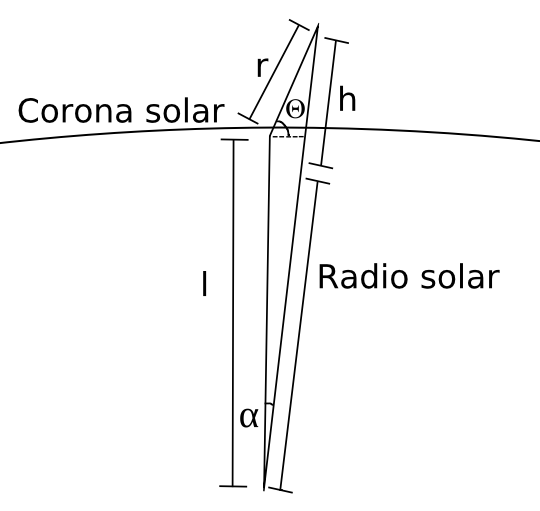
\includegraphics[scale=.8]{arco_magnetico_geometria}
\caption{ Representa la geometr\'ia que se utiliza para adaptar los par\'ametros del arco magn\'etico. }
\label{arco_geometria}
\end{figure}

\begin{figure}[h]
\centering
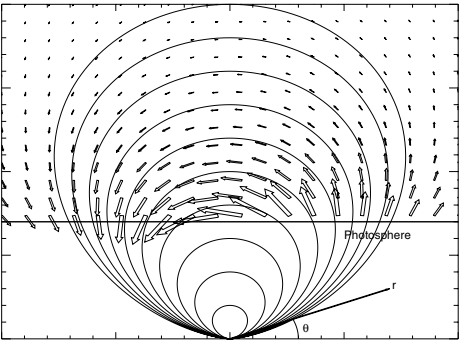
\includegraphics[scale=.8]{magnetic_loop}
\caption{ Imagen tomada del Aswanden. Representa el modelo de arco magn\'etico, donde la longitud de las flechas indican la intensidad del campo, y la direcci\'on en la que apuntan corresponde a la del campo. }
\label{arco_magnetico}
\end{figure}
\clearpage

\subsection{Flujo Emergente}

\textbf{Escala de altura (h). }Es un valor emp\'irico que permite determinar qu\'e tanto se difumina el campo magn\'etico con respecto a la altura. Su valor fue seleccionado de tal forma que los rangos de sus valores caigan dentro de los emp\'iricos que han sido observados. Concretamente, se tom\'o el valor de 200 debido a que arroja los resultados emp\'iricos observados, que van de 500 a 1000G \citep{VAULT}.*agregar referencia*

\textbf{Flujo magn\'etico (phi). }Representa el campo magn\'etico total que pasa por un \'area determinada. Para realizar las pruebas a la extensi\'on computacional propuesta, se tom\'o como valor del flujo magn\'etico $\phi=2.8x10^{18}$Mx. Si bien existe debate sobre las aproximaciones m\'as precisas con respecto a este valor \citep{magneticflux}; se consider\'o \'este debido a que los resultados del radio inicial del tubo de flujo del modelo de Flujo Emergente fueron coherentes con la teor\'ia (366km \citep{magneticflux} y \citep{VAULT}) al utilizarlo.

\textbf{Intensidad de campo inicial en su base (B0). }Se refiere al valor que toma el campo magn\'etico en la base, o desde el punto donde se desea comenzar a medir. Los c\'alculos fueron generados considerando distintos valores de campo magn\'etico (0, 500, 1000 y 1500 Gauss), dado que en la literatura se ha dado este valor entre 1000 y 1500 Gauss. La fuerza de la red cromosf\'erica es 1 kG a z=0 con una altura de 500km de acuerdo a Judge (2006 CORREGIR).

\clearpage
\section{Resultados}

En esta secci\'on se presentar\'an los resultados obtenidos de las simulaciones seg\'un los modelos de arcos magn\'eticos y flujo emergente.

\subsection{Micro arco magnetico}
El modelo de arcos magn\'eticos es uno de los modelos m\'as simples para simular el comportamineto solar. Sin embargo, a su vez, es un modelo que facilita la comprensi\'on y vizualicaci\'on de la morfolog\'ia del campo magn\'etico de una manera pedag\'ogica.

Los primeros resultados que se presentan, son aquellos concernientes a las pruebas de la codificaci\'on del modelo de arcos magn\'eticos para obtener lo perfiles de los propios arcos magn\'eticos. Particularmente, se realizaron pruebas en los campos magn\'eticos iniciales de 0, 25, 183 y 570G. Con estos valores se obtuvo un perfil del campo magn\'etico a lo largo de la altura; cuyos resultados se pueden apreciar en la Figura \ref{am_Campo_Magnetico}. Como se puede observar, los valores de los campos magn\'eticos arriba de los 1,000 km terminan siendo relativamente peque\~nos, independientemente del valor de entrada. Lo anterior va acorde a la teor\'ia del campo magn\'etico de la crom\'osfera.

Una vez obtenidos los perfiles de los arcos magn\'eticos, ya se puede ajustar la presi\'on de la crom\'osfera a diferentes alturas. Los resultados obtenidos a trav\'es de la extensi\'on al c\'odigo Pakal se representan en la Figura \ref{am_Presion}. En ella se puede ver que conforme m\'as grande es el campo magn\'etico, la presi\'on decrementa menos, manteni\'endose a un valor m\'as alto. 

Despu\'es de obtener los resultado de la presi\'on de la crom\'osfera, se pueden calcular los valores de la densidad del hidr\'ogeno presente en la crom\'osfera. Estos resultados se pueden apreciar en el gr\'afico \ref{am_perfil_de_densidades}. Como se puede observar el comporamiento general es que a mayor campo magn\'etico menor es el gradiente de la densidad. En adici\'on a estos resultados, se muestran tambi\'en dos comparativos entre los resultados de las densidades para diferentes campos magn\'eticos. Estos \'ultimos resultantes se grafican en la Figura \ref{am_diferencias_absolutas} y en la Figura \ref{am_diferencias_relativas}.

\newpage
\begin{figure}[h]
\centering
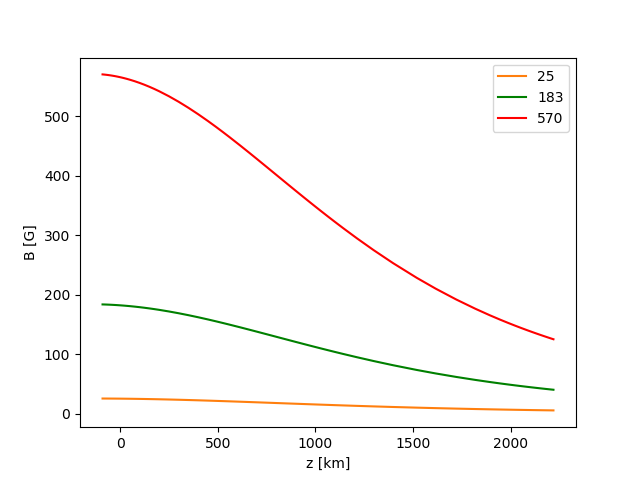
\includegraphics[scale=1]{am_Campo_Magnetico}
\caption{ En esta gr\'afica se describe el comportamiento de la intensidad del campo magn\'etico. }
\label{am_Campo_Magnetico}
\end{figure}


\begin{figure}[h]
\centering
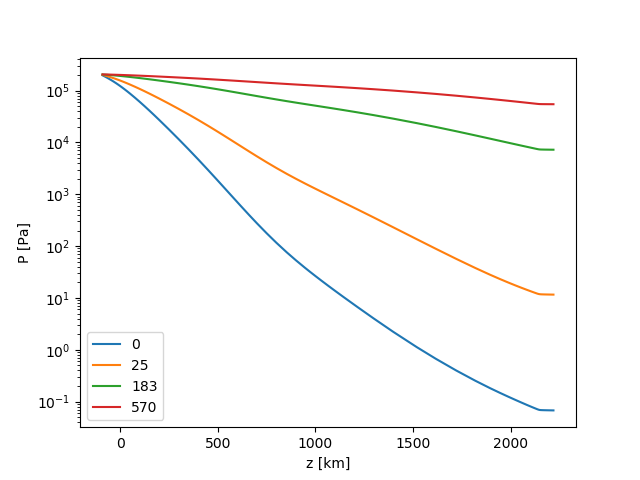
\includegraphics[scale=1]{am_Presion}
\caption{ Aqu\'i se presentan cada una de las salidas de las simulaciones con los distintos valores de campo magn\'etico seg\'un los resultados anteriores.}
\label{am_Presion}
\end{figure}

\begin{figure}[h]
\centering
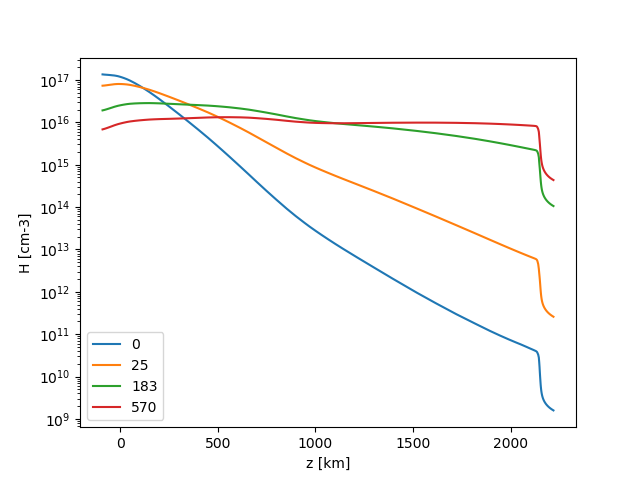
\includegraphics[scale=1]{am_perfil_de_densidades}
\caption{ En esta figura se grafican el perfil de densidades de hidr\'ogeno.}
\label{am_perfil_de_densidades}
\end{figure}

\begin{figure}[h]
\centering
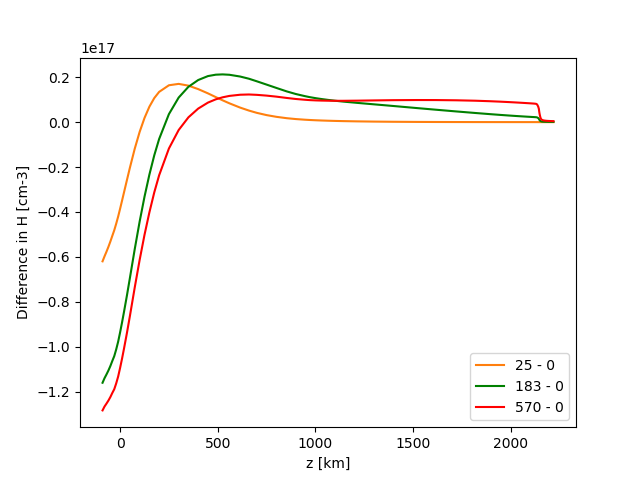
\includegraphics[scale=1]{am_diferencias_absolutas}
\caption{ Aqu\'i se muestra una comparaci\'on entre las diferentes salidas de las densidades del programa.}
\label{am_diferencias_absolutas}
\end{figure}

\begin{figure}[h]
\centering
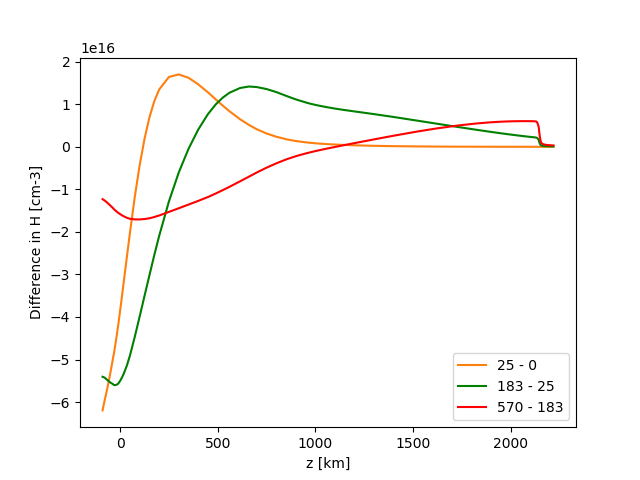
\includegraphics[scale=1]{am_diferencias_relativas}
\caption{ Aqu\'i se muestra un diferencial de cada uno de las salidas de las simulaciones contra las salidas de la simulaci\'on con un valor m\'as bajo.}
\label{am_diferencias_relativas}
\end{figure}


\clearpage
\subsection{Flujo emergente}
El m\'odelo de Flujo emergente es m\'as complejo que el modelo de arcos magn\'eticos, lo que lo hace f\'isicamente m\'as plausible. Sin embargo, es un modelo que no provee de explanantes a la generaci\'on de los campos magn\'eticos.

Al igual que con el modelo anterior. Primero se calcul\'o el perfil de los campos magn\'eticos seg\'un esta teor\'ia. Para esto, y como se explic\'o en secciones anteriores, se utilizaron los valores de 500, 1000 y 1500G. Como se puede apreciar en la Figura \ref{fe_Campo_Magnetico}, la intensidad del campo magn\'etico decae mucho m\'as r\'apido en comparaci\'on con el modelo anterior, a tal grado que para los 1,000km ya es pr\'acticamente despreciable su valor. Este fen\'omeno es a\'un m\'as acertado a las teor\'ias pertinentes.

Similarmente a lo realizado en el modelo de Flujo emergente, una vez obtenidos los valores del perfil de los campos magn\'eticos se procedi\'o a calcular la presi\'on cromosf\'erica. En este modelo se puede entrever un desplazamiento en la ca\'ida de la presi\'on de la crom\'osfera (V\'ease Figura \ref{fe_Presion}). A su vez, con este nuevo valor, se obtuvo el perfil de densidad, el cual presenta un desplazamiento en el gr\'afico para cada valor de campo. 
Finalmente, una vez obtenidos todos estos resultados, tambi\'en se procedi\'o a realizar dos comparativos entre los resultados de las diferentes perfiles de densidades. Los resultados de estas comparativas se pueden apreciar en la Figura \ref{fe_diferencias_absolutas} y Figura \ref{fe_diferencias_relativas}.

\begin{figure}[h]
\centering
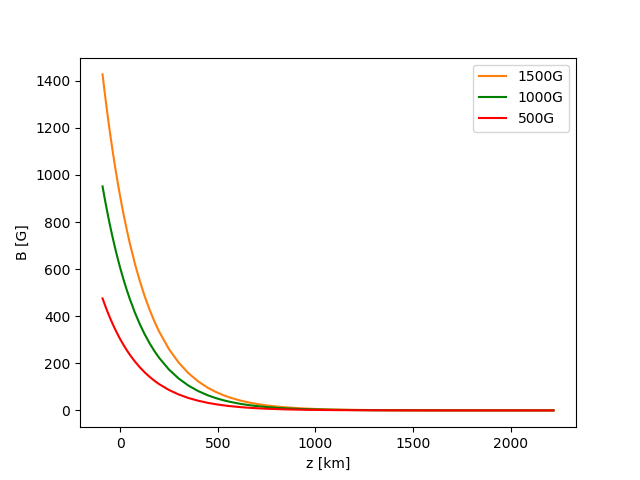
\includegraphics[scale=1]{fe_Campo_Magnetico}
\caption{ En esta gr\'afica se describe el comportamiento de la intensidad del campo magn\'etico. }
\label{fe_Campo_Magnetico}
\end{figure}

\begin{figure}[h]
\centering
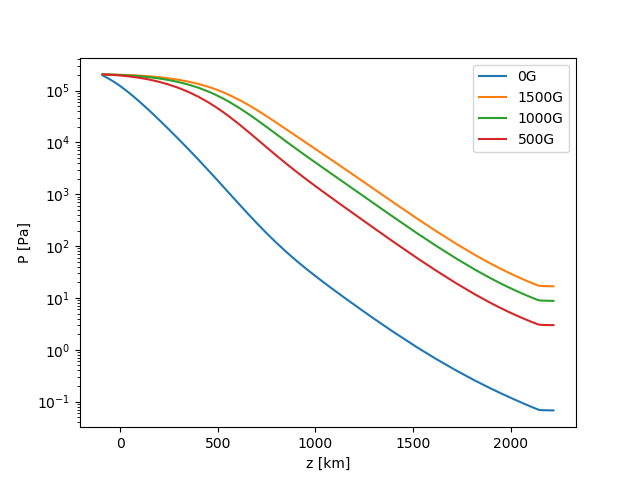
\includegraphics[scale=1]{fe_Presion}
\caption{ Aqu\'i se presentan cada una de las salidas de las simulaciones con los distintos valores de campo magn\'etico seg\'un los resultados anteriores.}
\end{figure}

\begin{figure}[h]
\centering
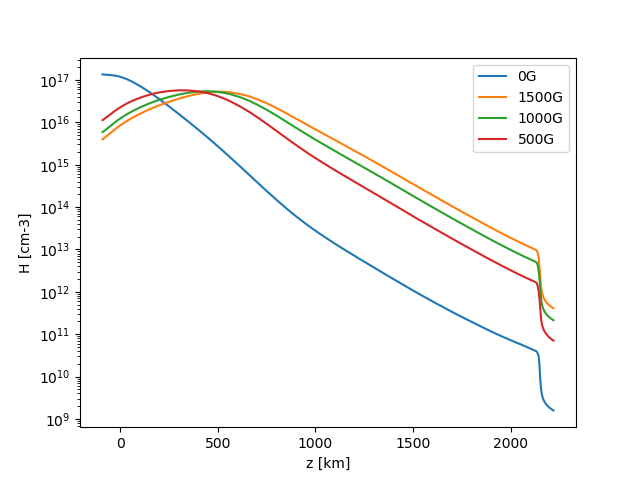
\includegraphics[scale=1]{fe_perfil_de_densidades}
\caption{ En esta figura se grafican el perfil de densidades de hidr\'ogeno.}
\label{fe_perfil_de_densidades}
\end{figure}


\begin{figure}[h]
\centering
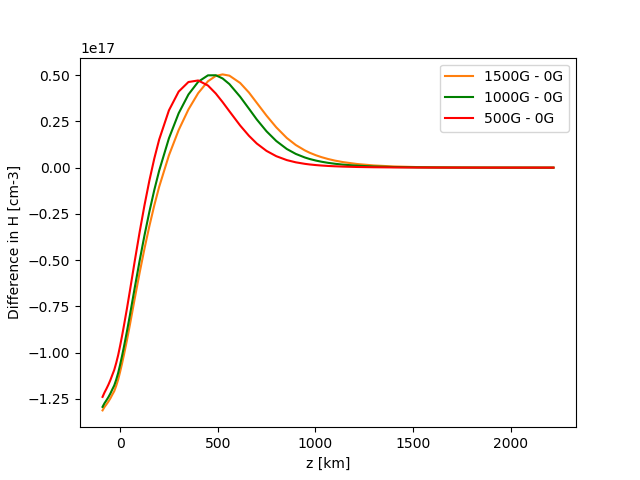
\includegraphics[scale=1]{fe_diferencias_absolutas}
\caption{ Aqu\'i se muestra una comparaci\'on entre las diferentes salidas de las densidades del programa.}
\label{fe_diferencias_absolutas}
\end{figure}

\begin{figure}[h]
\centering
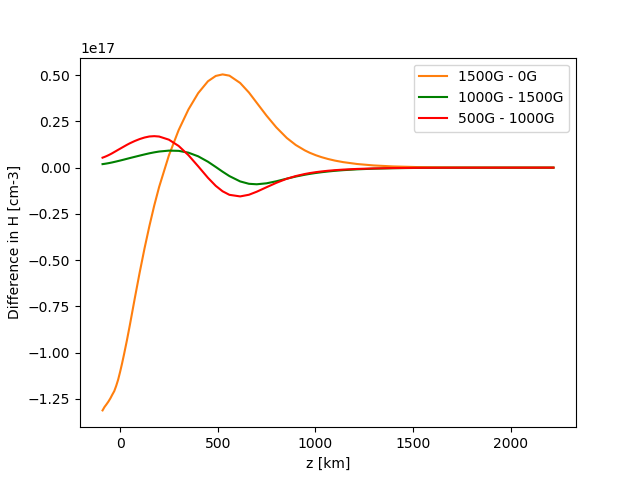
\includegraphics[scale=1]{fe_diferencias_relativas}
\caption{ Aqu\'i se muestra un diferencial de cada uno de las salidas de las simulaciones contra las salidas de la simulaci\'on con un valor m\'as bajo.}
\label{fe_diferencias_relativas}
\end{figure}
\clearpage
